\newchapstyle
\chapter{Introduction}
\label{chap:intro}

%\epigraph[0pt]{
%    Failure is not an option.
%}{Actor Ed Harris, playing flight director Gene Kranz, in the 1995 film Apollo 13\cite{FailureNotOption2019}}

%\begin{abstract}
%Lorem ipsum dolor sit amet, consectetur adipisicing elit, sed do eiusmod tempor incididunt ut labore et dolore magna aliqua. Ut enim ad minim veniam, quis nostrud exercitation ullamco laboris nisi ut aliquip ex ea commodo consequat. Duis aute irure dolor in reprehenderit in voluptate velit esse cillum dolore eu fugiat nulla pariatur. Excepteur sint occaecat cupidatat non proident, sunt in culpa qui officia deserunt mollit anim id est laborum.
%\end{abstract}

%% Start the actual chapter on a new page.
\afterpage{\pagecolor{none}}\newpage

\section{Computing with semi- and superconducting circuits}

The invention of the metal oxide semiconductor field-effect transistor (MOSFET, cf. Fig.~\ref{fig:introcomputing}(a)) lay the ground to the information age, in large parts shaping the world to be what we know it as today.
%
Pushed by continuous advances in material sciences, solid state physics and electrical engineering, the MOSFET is now the building block of all commercial computers.
%
Owed largely by the success of scalability from integrated circuits, today's state-of-the-art microprocessors can host more than 39.54 billion transistors on a single chip, with physical dimensions down to a few tens of nanometers, cf. Fig.~\ref{fig:introcomputing}(b)~\cite{mujtabaAMDEPYCRome2019}.
%
With the increasing transistor density and shrinking physical dimensions came however the realization, that alternative computation architectures to the one based on semiconducting transistors might be needed to satisfy society's desire for computation power, as there might be a limit to how dense logic circuits could be packed with current technology.
%
The slowing of Moore's law, originally predicting the doubling of transistor chip density every two years~\cite{mooreCrammingMoreComponents2006}, is an important reminder of this challenge.


Already before the invention of the MOSFET, circuits on the basis of superconducting switches called "cryotrons" were envisioned as a competitive alternative to semiconducting computers~\cite{buckCryotronASuperconductiveComputer1956,brockWillNSAFinally}.
%
The discovery of Josephson junctions (JJs), weak links between two superconductors, depicted in Fig.~\ref{fig:introcomputing}(e), in 1962~\cite{josephsonPossibleNewEffects1962,andersonProbableObservationJosephson1963} spured additional interest due to their sensitive nature to magnetic flux, low power consumption and high switching speeds~\cite{mcdonaldPicosecondApplicationsJosephson1980}.
%
In parallel to the development of MOSFETs, Josephson junctions were hence envisioned as building blocks for superconducting logic circuits, with IBM being one of the main drivers at the time~\cite{anackerJosephsonComputerTechnology1980a}.
%
In an attempt to combine the best of two worlds, the versatility of a high gain transistor, and the low dissipation of superconducting circuits, proposals were made in the 1980s to merge these two elements into the Josephson field effect transistor (JoFET), cf. Fig.~\ref{fig:introcomputing}(c)~\cite{clarkFeasibilityHybridJosephson1980,gallagherThreeterminalSuperconductingDevices1985}.


While IBM eventually seized to research Josephson junction computation due to an apparent supremacy of semiconducting computers~\cite{robinsonIBMDropsSuperconducting1983}, research continued at public institutions and universities, in part driven by Richard Feynman's ideas of building quantum machines to run complex calculations much more efficient than any classical, MOSFET-based, computer~\cite{feynmanSimulatingPhysicsComputers1982}.
%
The late twentieth century then saw the birth of first prototypes for a quantum computing architecture, and it was realized that Josephson junctions could form the basis of quantum bits~\cite{martinisQuantumJosephsonJunction2020}.
%
Since then, global tech companies like IBM, Google, Microsoft and Intel are all heavily invested in this architecture, each following a slightly different path~\cite{steffenQuantumComputingIBM2011,aruteQuantumSupremacyUsing2019,linnNewMicrosoftBreakthroughs2020,vandersypenQuantumComputingSemiconductor2019}.
%
Superconducting quantum processors based on Josephson junctions embedded in microwave circuits, as pursued by IBM and Google, have culminated in the milestone "quantum supremacy", i.e. the threshold at which a quantum processor can execute an algorithm that would be prohibitively costly in terms of computing time and money for a classical computer to perform~\cite{aruteQuantumSupremacyUsing2019}.
%
Figure~\ref{fig:introcomputing}(e) shows an image of Google's "quantum supremacy" processor.
%
The building block of these processors are transmon qubits.
%
These consist of a coplanar capacitance in series with superconducting quantum interference devices (SQUIDs), formed by two Josephson junctions in a loop.



To tune the states of the transmons, magnetic flux is threaded through the SQUID loop, supplied via on-chip current bias lines in close proximity to the SQUIDs.
%
While coherence times of several hundreds of microseconds show great potential for future devices~\cite{placeNewMaterialPlatform2020}, standard transmons come with a few drawbacks:
%
Already the very first implementation of a two-qubit transmon processor showed that magnetic fields can lead to significant cross talk coupling qubits several centimeters apart from each other\cite{dicarloDemonstrationTwoqubitAlgorithms2009}.
%
Additionally, since the chips need to be operated at temperatures only fractions of a Kelvin above absolute zero in order to protect their coherence from thermal excitations, the cooling power of the refrigerator must not be exceeded.
%
This can be problematic with high qubit numbers, since the tuning current through all individual flux lines might exceed the cooling power.
%
As the number of physical qubits increases, so does the challenge of shielding individual qubits from each other's bias lines, and retaining enough cooling power as to not induce thermal effects.

In contrast, replacing SQUIDs with the long-abandoned JoFET might be beneficial:
%
Applying gate voltages instead of running a current through a wire does not lead to thermal dissipation, which removes the cooling power constraint.
%
Additionally, cross-talk can be significantly reduced due to the nature of electric fields in gate capacitors being strongly confined to a small volume around the gate voltage lead.
%
Finally, JoFETs have consistently performed well under application of in-plane magnetic fields.
%
While the latter are not strictly necessary in transmon qubits (rather to be avoided) flux noise is one of the limiting factors of SQUIDs, to which gatemons are insensitive~\cite{casparisSuperconductingGatemonQubit2018}.
%
Even more important, magnetic field-compatible JoFETs are one of the requirements of qubits based on the Majorana architecture, which could result in significantly more coherent qubits due to their intrinsic topological protection~\cite{hyartFluxcontrolledQuantumComputation2013}.


\begin{figure}[t]
	\centering
	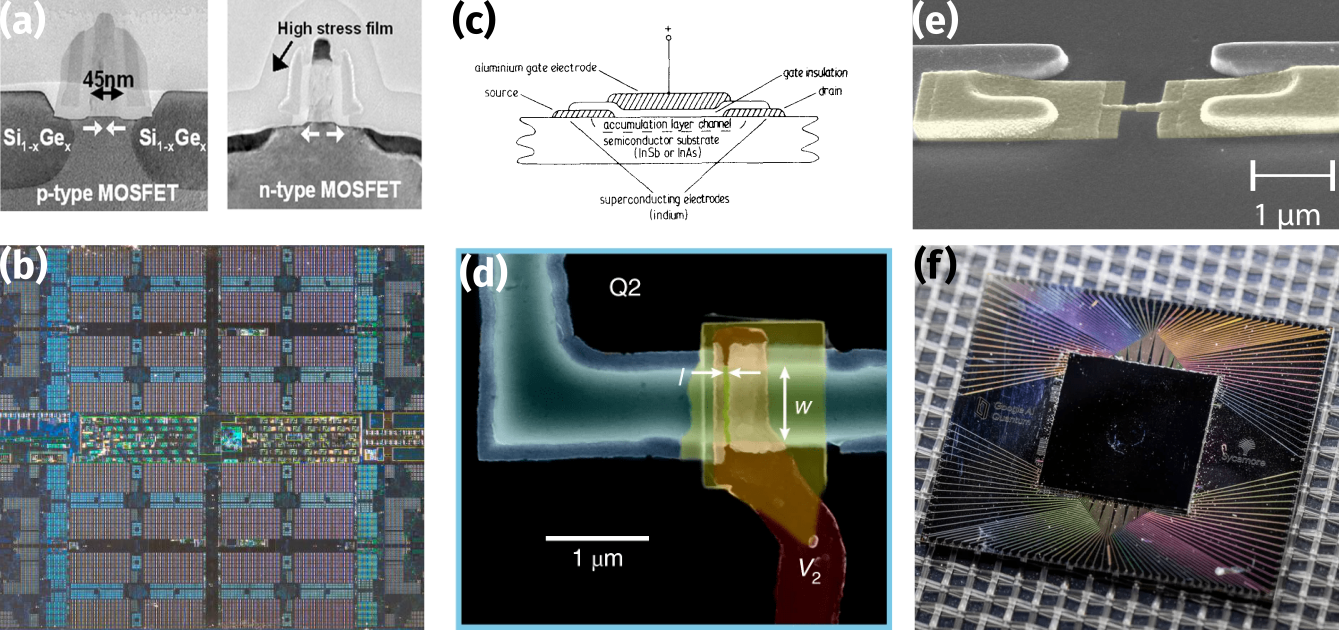
\includegraphics[width=\linewidth]{chapter-introduction/figs/intro_computing.svg.png}
	\caption{
		\textbf{Semi- and superconducting based computing devices.}
		%
		\textbf{(a)} Cross-sectional TEM image of \SI{45}{\nano\meter} node MOSFETs, the building block of semiconducting computers.
		%
		Figure adapted from~\cite{thompsonLogicNanotechnologyFeaturing2004}.
		%
		\textbf{(b)} Die shot of part of the I/O die of the microprocessor with currently highest number of transistors, in this case with \SI{14}{\nano\meter} node: The \textit{AMD Epyc Rome} with \num{8.34} billion transistors on the I/O die and \num{39.54} billion in total.
		%
		Figure adapted from \cite{fritzAMD7nm12nmIOD2019}.
		%
		\textbf{(c)} Sketch of the first envisioned JoFET as hybrid between semiconducting transistors and superconducting Josephson junctions.
		%
		Figure adapted from~\cite{clarkFeasibilityHybridJosephson1980}.
		%
		\textbf{(d)} SEM of a gatemon qubit, a potential building block for quantum computing on a hybrid super-semi approach.
		%
		Figure adapted from~\cite{casparisSuperconductingGatemonQubit2018}.
		%
		\textbf{(e)} SEM of an aluminum oxide Josephson junction, the workhorse of state-of-the-art superconducting microwave quantum  computing.
		%
		Figure adapted from~\cite{langfordExperimentallySimulatingDynamics2017}.
		%
		\textbf{(f)} Optical image of Google's "quantum supremacy" 53 qubit \textit{Sycamore} quantum processor.
		%
		Figure adapted from~\cite{shanklandTakeLookGoogle2020}. 
	}
	\label{fig:introcomputing}
\end{figure}

As of now, there has been only very little research in integrating JoFETs in superconducting quantum computing.
%
Recently, semiconductor nanowires and epitaxial 2DEGs were incorporated in transmon qubits, resulting in so-called "gatemons", cf. Fig.~\ref{fig:introcomputing}(d)~\cite{delangeRealizationMicrowaveQuantum2015,larsenSemiconductorNanowireBasedSuperconductingQubit2015,casparisGatemonBenchmarkingTwoQubit2016a,casparisSuperconductingGatemonQubit2018,luthiEvolutionNanowireTransmon2018}.
%
While coherence times are not yet at the same level as for standard transmons, gatemons show great promise and have gained significant interest in the scientific community.
%
They not only provide a new way of qubit control~\cite{shimSemiconductorinspiredDesignPrinciples2016}, but also a path towards studying unconventional superconducting weak links at high frequencies~\cite{tahanGrapheneQubitMotivates2019}.





In this thesis, we initially set out to explore how JoFETs based on graphene Josephson junctions (gJJs) could perform in superconducting microwave circuits.
%
Since its discovery in 2004, graphene has shown versatile field effect applications and, already since very early on, gate-tunable superconductivity~\cite{novoselovElectricFieldEffect2004c,heerscheBipolarSupercurrentGraphene2007a}.
%
With improvements in contact engineering and reduced film disorder, induced superconductivity in gJJs has been a testbed for Andreev physics, phase coherent mechanisms, quantum phase transitions and the interplay of superconductivity and magnetism ~\cite{leeProximityCouplingSuperconductorgraphene2018a}.
%
Integrating gJJs in microwave circuits would thus be a first step towards the realization of gate-tunable superconducting microwave logic circuits.
%
In order to retain information about the device's DC properties, and to directly link them to the microwave performance, we chose to combine both DC and MW in one device.
%
To this end, we based our circuits on an architecture that allows simultaneous signal probing both with low and high frequencies, DC bias microwave cavities~\cite{bosmanBroadbandArchitectureGalvanically2015c}.
%
This not only allows for a detailed study of the junction's properties, but also enables applications based on current-biasing the sample.







\section{Josephson effects in SNS systems}

Josephson junctions are formed by a weak link between two superconducting electrodes, which mus be sufficiently weak to sustain a phase difference $\delta=\phi_1-\phi_2$ between the phases of the two electrodes, $\phi_1$ and $\phi_2$, respectively.
%
The perhaps simplest case of a JJ is a thin insulating tunnel barrier between two superconductors, the SIS JJ, cf. Fig.~\ref{fig:modelsnsdos}(a).
%
Here, Cooper pairs can tunnel from one superconductor through the barrier to the other side, while acquiring a phase $\delta$.
%
The current flowing across this type of junction is given by
%
\begin{align}
I_J^{\rm SIS}(\delta) &= I_c\sin\delta.
\end{align}

The situation is different in the case in which the weak link consists of a normal metal between two superconducting banks, an SNS junction.
%
To support a supercurrent, the length of the normal metal must be smaller than the coherence length in the normal region, $L<\xi_N$, which in fact is much longer than the maximum thickness of the insulating barrier in the case of an SIS junction, where the thickness has to be smaller than the superconducting coherence length, $t\ll\xi_S$~\cite{caladoBallisticJosephsonJunctions2015d,benshalomQuantumOscillationsCritical2015}.
%
The process of Andreev reflection at the interface between superconductors and normal metals lays the basis for understanding how an SNS junction works~\cite{blonderTransitionMetallicTunneling1982c}.
%
The process is sketched in Fig.~\ref{fig:modelsnsdos}(b):
%
An electron impinging onto the super-normal interface from inside the normal region can only enter the superconductor in the form of a Cooper pair by being reflected as a hole with opposite spin and momentum.
%
Vice versa, a Cooper pair travelling towards the normal region will decay into an electron travelling forward, and annihilate a hole travelling backwards with spin opposite to that of the electron.
%
Inside the normal region, this will result in the formation of the so-called Andreev bound states (ABS) and a net current across the JJ.

\begin{figure}[t]
	\centering
	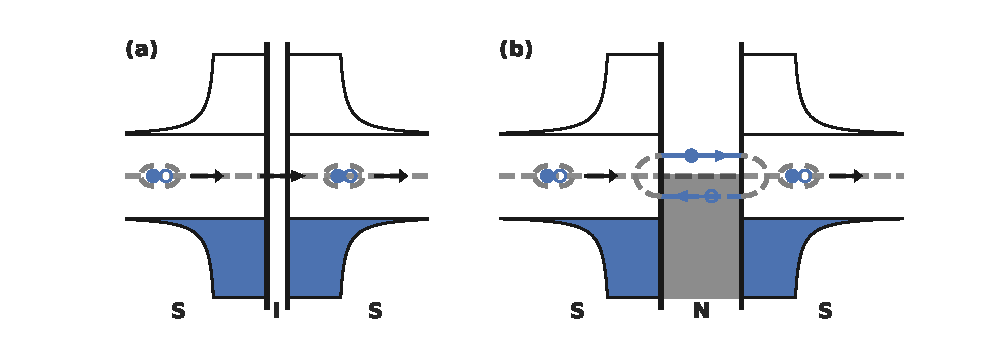
\includegraphics[width=\linewidth]{chapter-introduction/figs/model_SNS_DOS}
	\caption{
		\textbf{Cooper pair transport in SIS and SNS Josephson junctions.}
		%
		The density of states in a superconductor exhibits a gap of width $2\Delta$ in energy around the Fermi level $\epsilon_F$, with states below $\epsilon_F$ filled and states above unoccupied.
		%
		\textbf{(a)} In an SIS Josephson junction, Cooper pairs, consisting of an electron and hole with opposite spins and momentum, can tunnel through a thin insulating barrier separating two superconducting banks.
		%
		There are no states inside the insulating region.
		%
		\textbf{(b)} In an SNS Josephson junction, the normal region exhibits a DOS that is filled up to $\epsilon_F$.
		%
		Unpaired electrons can enter the superconductor by Andreev reflection as a hole with opposite momentum.
		%
		Conversely, Cooper pairs can enter the normal region by breaking into an electron and hole of opposite spin and momentum.
		%
		This way, Andreev bound states form within the normal region and a net current flows across the junction.
	}
	\label{fig:modelsnsdos}
\end{figure}


The current-phase relation in SNS junctions takes on a significantly different form than the sinusoidal one in SIS junctions:
%
For the simplest case of a one-dimensional SNS junction with perfect contact transparency $\tau_c=1$ at the SN interface, each Andreev bound state has a ground state energy
%
\begin{align}
E_{i}^{\rm ABS} = -\Delta\sqrt{1-T_i\sin^2(\delta/2)}
\label{eq:ABS}
\end{align}
%
with induced superconducting gap $\Delta$ and channel transparency $T_i$, where $T_i$ takes into account scattering inside the normal region\cite{beenakkerUniversalLimitCriticalcurrent1991,titovJosephsonEffectBallistic2006b}.
%
The energy of the excited ABS has opposite sign.
%
Summing over all channels in the junction, the total Josephson potential is given by
%
\begin{align}
U_J(\delta) = 1-\sum_i E_{i}^{\rm ABS} \approx E_J \frac{\delta^2}{2} - E_J\left( 1-\frac{3\sum T_i^2}{4\sum T_i} \right) \frac{\delta^4}{24} +\mathcal{O}(\delta^6)%\ , \\
%E_J &= \frac{\Delta}{4}\sum_i T_i \rightarrow \frac{\Delta}{4}N\tau
\end{align}
%
where we Taylor-expanded Eq.~\ref{eq:ABS}~\cite{kringhojAnharmonicitySuperconductingQubit2018}.
%
In the limit of low $T_i$, i.e. for an SIS junction, the energy would be given simply by $U_J^{\rm SIS}(\delta)=1-E_J\cos(\delta)\approx E_J\delta^2/2-E_J\delta^4/24$.
%
Compared to the SIS case, we therefore find that the Josephson energy is reduced by a fraction depending on the channel transparency which will become important for gatemon qubits, cf. Ref.~\cite{kringhojAnharmonicitySuperconductingQubit2018} and Chapter~\ref{chap:gJJ-CPR}.
%
We plot the ground and excited state energies of the ABS in Fig.~\ref{fig:modelsnsejic}(a).
%
With increasing channel transmission, $U_J$ exhibits stronger modulation and a closing band gap at $\delta=\pi$ with minimum separation $2\Delta\sqrt{1-\tau}$.

The corresponding relation between Josephson current and the respective phase drop across the one-dimensional SNS JJ is 
\begin{align}
I(\delta) = \frac{2e}{\hbar}\frac{\partial U_J}{\partial\delta} = \frac{e\Delta}{2\hbar}\sum_i\frac{T_i\sin\delta}{\sqrt{1-T_i\sin^2\delta/2}}
\end{align}

In addition, we can ascribe an inductance value to the JJ, given by
%
\begin{align}
L_J(\delta) &= \frac{\hbar}{2e}\left( \frac{\partial I_J}{\partial\delta} \right)^{-1} = \left(\frac{\hbar}{2e}\right)^2\left(\frac{\partial^2U_J}{\partial\delta^2}\right)^{-1} \nonumber\\
&= \frac{4\hbar^2}{e^2\Delta}\sum_i \frac{\left(1-T_i\sin^2(\delta/2)\right)^{3/2}}{4T_i\cos\delta\left(1-T_i\sin^2(\delta/2)\right)+T_i^2\sin^2(\delta)}
\end{align} 
%
In the microwave regime, the junction therefore behaves as a strong nonlinear inductor.

Both quantities are depicted in Fig.~\ref{fig:modelsnsejic}(b,c).
%
We can conclude two things:
%
First, the larger the channel transmission, the stronger the forward skew of the current phase relation and corresponding deviation to the SIS case.
%
Second, while also strongly nonlinear, the Josephson inductance of SNS junctions is significantly reduced compared to the SIS case, $L_J^{\rm SIS}=\hbar(2eI_c\cos\delta)^{-1}$.
%
Since exact knowledge of the Josephson inductance is critical for operating transmon qubits, these deviations need to be investigated for future applications. 

\begin{figure}[t]
	\centering
	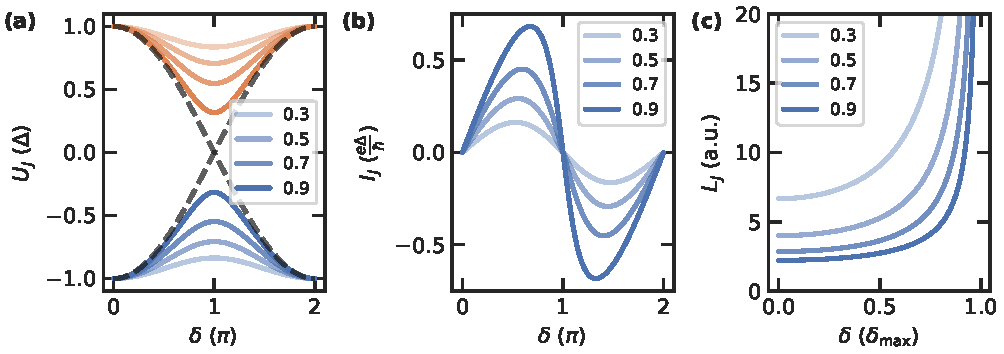
\includegraphics[width=\linewidth]{chapter-introduction/figs/model_SNS_EjIc}
	\caption{
		\textbf{Channel transmission and nonsinusoidality.}
		%
		\textbf{(a)} Josephson energy of the ground (blue) and excited (orange) Andreev bound state for varying channel transmission $\tau$ as a function of phase drop across the Josephson junction.
		%
		Increasing color intensity corresponds to increasing $\tau$.
		%
		Dashed line indicates the bulk gap $\pm\Delta$.
		%
		\textbf{(b)} Josephson current for varying $\tau$.
		%
		Increasing transmission increases both amplitude and forward skewing of the CPR.
		%
		\textbf{(c)} Josephson inductance as a function of phase normalized to the one at maximum $L_J$.
		%
		Due to the increased CPR slope for increasing $\tau$ around $\delta=0$, the Josephson inductance decreases significantly.
	}
	\label{fig:modelsnsejic}
\end{figure}

However, for a realistic SNS junction such as the two-dimensional graphene devices measured in this thesis, there are a number of effects that lead to deviations of the above presented mechanisms.
%
The exact nature of the subgap density of states for example depends on size and geometry of the junction, as well as the contact transparency.
%
If the junction is sufficiently wide that the transport is no longer strictly one-dimensional, the ABS energy is reduced and moves closer to zero.
%
The same holds for the case of long compared to short junctions, cf. Fig.~\ref{fig:modelsubgap}:
%
This can be understood qualitatively by an effective energy $E_{\rm Th^\star}=\hbar v_F/\Lambda<\Delta$ governing transport inside the junction, analogously to the Thouless energy~\cite{benshalomQuantumOscillationsCritical2015,schmidtBallisticGrapheneSuperconducting2018}, with an effective length scale $\Lambda=L/\tau$ and the Fermi velocity $v_F$.
%
In the case of a very wide junction, the transverse Thouless energy $E_{\rm Th^\star}^\parallel=\hbar v_F/\Lambda_\parallel$ with $\Lambda_\parallel=W/\tau$ needs to be introduced.
%
The lower this energy, the longer the dwell time of ABS inside the normal region, hence their lower energy.
%
Finally, reduced contact transparency $\tau_c<1$ at the SN interface leads to the ABS detaching from the bulk gap at $\Delta$ even for zero phase difference~\cite{bretheauTunnellingSpectroscopyAndreev2017a}.


Figure~\ref{fig:modelsubgap} shows the calculated subgap density of states (DOS) for a exemplary graphene Josephson junction in the short and long regime, i.e. $L_N\ll\xi$ and $L_N>\xi$.
%
We find that for both cases the states with lowest energies are located at large parallel momentum $k_\parallel$, and that for the long junction, there are a number of subgap states below the bulk gap energy $\Delta$.
%
This significantly induced gap can potentially absorb RF excitations, leading to dissipation and decoherence in microwave circuits.
%
Finally, graphene shows strong angle-dependent transport due to Klein-tunneling at interfaces, which collimates charge carrier transport perpendicular to interfaces at pn junctions, which can further modify the DOS~\cite{beenakkerColloquiumAndreevReflection2008}.

\begin{figure}[t]
	\centering
	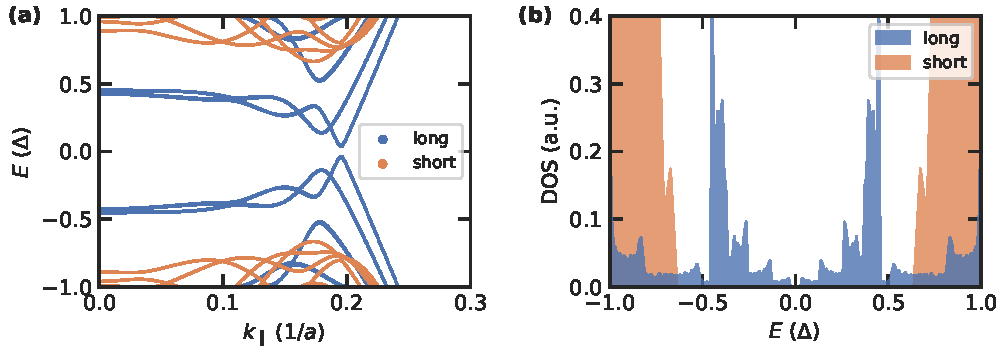
\includegraphics[width=\linewidth]{chapter-introduction/figs/kwant_modeling_181206_subgap_length_supp_Plot_subgap_dos}
	\caption{
		\textbf{Realistic subgap states of a 2D graphene Josephson junction.}
		%
		Tight-binding simulations of a graphene Josephson junction show strong dependence of the subgap state energies on momentum parallel to the SN interface \textbf{(a)}, with lowest lying energies at large $k_\parallel$.
		%
		While the short JJ (orange) shows an only slightly reduced minimum energy and DOS \textbf{(b)} compared to $\Delta$, long junctions (blue) exhibit heavily reduced energy gaps.
	}
	\label{fig:modelsubgap}
\end{figure}

In order to build reliable, reproducible circuits out of SNS junctions, it is thus vital to characterize them not only in the DC, but also in the microwave regime, as this is where the inductance will be measurable.
%
To this end, we placed our junctions in a circuit allowing for steady and high frequency signals to probe our device.
%
These DC bias microwave circuits are described in the following section.

\section{DC bias cavities for probing Josephson junctions}

\begin{figure}[t]
	\centering
	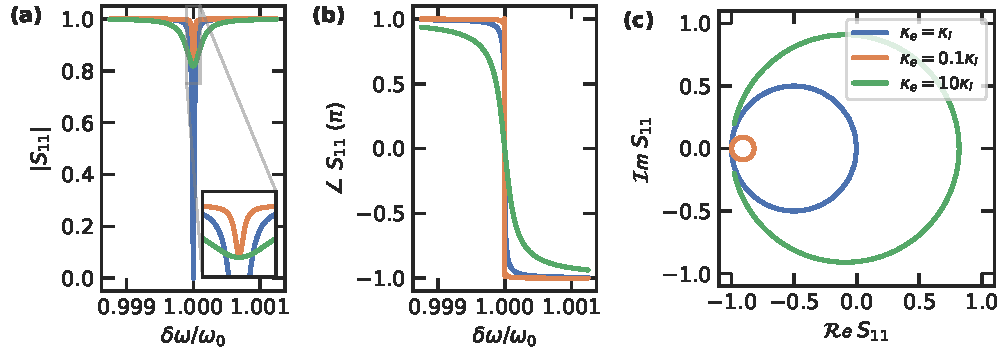
\includegraphics[width=\linewidth]{chapter-introduction/figs/model_DC_bias_cavity_coupling.pdf}
	\caption{
		\textbf{Effect of coupling ratio of the reflection coefficient of a DC bias cavity.}
		%
		Using Eq.~\ref{eq:intro-s11}, we can model the absolute value \textbf{(a)}, phase \textbf{(b)} and real and imaginary parts \textbf{(c)} of the reflection coefficient of a DC bias cavity.
		%
		Colors denote the various coupling types: blue: critically coupled $\kappa_e/\kappa_i=1$, orange: undercoupled $\kappa_e/\kappa_i=0.1$, green: overcoupled $\kappa_e/\kappa_i=10$.
		%
		Best signal-to-noise ratio in terms of $\abs{S_{11}}$ is achieved for critical coupling, while the other two cases have identical SNR.
	}
	\label{fig:s11}
\end{figure}


To probe the Josephson inductance, we make use of superconducting microwave resonators based on coplanar waveguides~\cite{gopplCoplanarWaveguideResonators2008,zmuidzinasSuperconductingMicroresonatorsPhysics2012}.
%
These have been used extensively in the field of particle detection and circuit (quantum) electrodynamics due to their intrinsic low loss originating from the absent resistance of the Cooper pairs~\cite{dayBroadbandSuperconductingDetector2003a,blaisCavityQuantumElectrodynamics2004c,clerkHybridQuantumSystems2020,blaisQuantumInformationProcessing2020}.
%
For probing the device under test both in the low and high frequency range (DC to several $\SI{e9}{\hertz}$), our circuits need to sustain a stable resonance when biased with direct currents.

There is a variety of circuit architectures capable of this approach, such as using inductive coupling~\cite{vissersFrequencytunableSuperconductingResonators2015b}, direct leads at voltage nodes of a $\lambda/2$ resonator with matching length~\cite{chenIntroductionDcBias2011a,liApplyingDirectCurrent2013} or lumped-element split-cavities~\cite{mahashabdeFastTunableHigh2020}.
%
In contrast, we based our design on an architecture previously developed in our group: the shunt capacitor DC bias cavity~\cite{bosmanBroadbandArchitectureGalvanically2015c}.
%
This circuit has several advantages over the previously mentioned ones:
%
As no circuit symmetries need to be considered, the circuit layout is rather simple.
%
Because the shunt capacitor is placed at the input port to the device, no additional port needs to be used to probe or excite the DUT, which prevents additional leakage channels.
%
Finally, using a shunt capacitor provides a broadband signal port up to the self-resonance of the shunt capacitor, which is chosen to be well above the resonance frequency of the circuit.

Figure~\ref{fig:TLmodel}(a) depicts a schematic of the DC bias cavity circuit.
%
In principle, measurements in both transmission and reflection geometry are possible.
%
However, we typically use the second port for supplying a DC gate voltage, and short the DUT to ground.
%
Therefore, we only perform reflection measurements.
%
The reflection coefficient of this circuit is given by
%
\begin{align}
S_{11}=-1+\frac{2\kappa_e}{\kappa_e+\kappa_i+2i\Delta}
\label{eq:intro-s11}
\end{align}
%
with the internal and external loss rates $\kappa_i$ and $\kappa_e$ and the detuning $\Delta=\omega-\omega_0$~\cite{bosmanBroadbandArchitectureGalvanically2015c}.
%
In Fig.~\ref{fig:s11} we plot the reflection coefficient for various fractions of $\eta =\kappa_e/\kappa_i$, to illustrate the effects of over-, under- and critical coupling ($\eta >1$, $\eta <1$ and $\eta =1$, respectively).
%
For a best signal-to-noise ratio in terms of $\abs{S_{11}}$, the shunt capacitor $C_s$ should be designed such that $\kappa_e=\kappa_i$, with the external loss rate approximately given by
%
\begin{align}
\kappa_e &= \frac{\omega_0}{Q_e} = \frac{2}{\pi\omega_0Z_0^2C_s^2}
\label{eq:intro-kappae}
\end{align}
%
with external quality factor $Q_e$ and transmission line impedance $Z_0$.
%
Due to stray inductance of the shunt capacitor, there is an upper limit to the maximum feasible $C_s$ we can use while keeping the self-resonance of the latter well above $\omega_0$.
%
In practice, this limits $Q_e$ to approximately \num{100e3}.
%
However, when placing a JJ at the end of the TL, the internal loss rate can rise significantly.
%
For this reason, we typically design our circuits such that they would be overcoupled in the case of a short to ground instead of a JJ, anticipating a rise in $\kappa_i$.


\begin{figure}
	\centering
	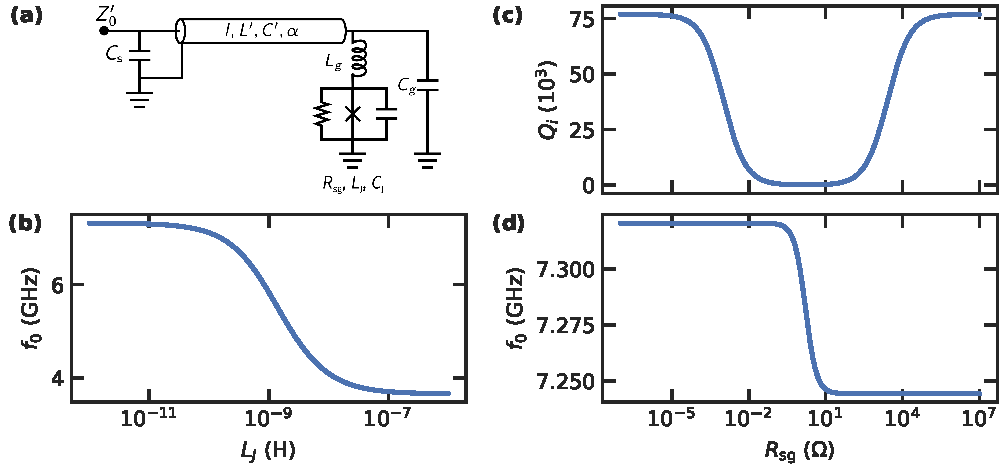
\includegraphics[width=\linewidth]{chapter-introduction/figs/model_DC_bias_cavity_params_RCSJ.pdf}
	\caption{
		\textbf{DC bias cavity shorted to ground by a parametrized top-gated graphene Josephson junction.}
		%
		\textbf{(a)} Fully parametrized circuit model.
		%
		The transmission line is described by length $l$, inductance and capacitance per unit length $L^\prime$ and $C^\prime$ and attenuation $\alpha$, and is coupled to an input impedance $Z_0^\prime$ via a shunt capacitance $C_s$.
		%
		The Josephson junction is modeled as a network of linear lead inductance $L_g$ together with an RCSJ model of subgap-resistance $R_{\rm sg}$, junction capacitance $C_J$, nonlinear inductance $L_J$ and gate capacitance $C_g$.
		%
		\textbf{(b)} Resonance frequency versus Josephson inductance with the other parameters fixed.
		%
		Depending on the junction impedance, the fundamental cavity mode changes from $\lambda/2$ (small $L_J$) to $\lambda/4$ (large $L_J$).
		%
		\textbf{(c,d)} Influence on subgap resistance on internal quality factor and resonance frequency.
		%
		Small $R_{\rm sg}$ corresponds to a short, large $R_{\rm sg}$ to an open to ground in parallel to $L_J$.
		%
		In both cases, the internal losses of the circuit are dominated by the transmission line attenuation.
		%
		For intermediate values of $R_{\rm sg}$, significant resistive damping effectively suppresses the circuit response.
		%
		Panel \textbf{(d)} also illustrates the shift of $f_0$ when changing the boundary condition of the circuit, similar to the on due to $L_J$ in panel \textbf{(b)}.
	}
	\label{fig:TLmodel}
\end{figure}


When probing Josephson junctions with the DC bias cavity, we need to calibrate the parameters of the microwave circuit prior to extract quantitative information on the high frequency properties of the added JJ.
%
We do this by measuring a combination of open and shorted references device with the same sample geometry, except with an open or short to ground in place of the JJ.
%
Equipped with these values, we can proceed to study the influence JJ on the microwave circuit:
%
With an added Josephson junction with inductance $L_J$ shorting the TL to ground, the shifted resonance frequency can be approximated by
%
\begin{align}
\omega_0^\prime = \omega_0\frac{L_r+L_J}{L_r+2L_J}
\label{eq:intro-omega0p}
\end{align}
%
where $L_r$ is the lumped TL resonator inductance including geometric and kinetic inductances, cf. Chapter~\ref{chap:gJJ-CPR} and Fig.~\ref{fig:TLmodel}(b).
%
A complete analytical model of an RSCJ model parametrizing the JJ can be used for calculating junction-induced losses in the form of a subgap resistance, cf. Chapter~\ref{chap:gJJ} and Fig.~\ref{fig:TLmodel}.
%
For very small $R_{\rm sg}$, the Josephson inductance is effectively short-circuited, so both $Q_i$ and $f_0$ approach the limit of no JJ.
%
On the other hand, very large $R_{\rm sg}$ implies an open circuit with no losses other than the ones in the TL resonator, again approaching $Q_i$ of the bare cavity and $f_0$ shifting the the value due to the added $L_J$.
%
Intermediate resistance values suppress the resonance entirely.
%
The shift in $f_0$ for large $R_{\rm sg}$ shows the frequency shift induced by $L_J$.



\section{Outline}

In the following, we will show how DC bias cavities can be utilized to both extract information on the intrinsic microwave properties of a Josephson junction, and use the combination of cavity and junction to detect very small currents.

In chapter~\ref{chap:experiment}, we provide an overview on the experimental methods that we developed and used to enable the measurements presented later on.
%
We detail the exfoliation and fabrication of graphene and boron nitride, and the fabrication of gJJs and superconducting CPW resonators.
%
Additionally, a short introduction to the use of the superconducting alloy molybdenum-rhenium in Delft, together with a small study on its pros and cons, is supplied.
%
The chapter closes with a brief introduction to thermal noise and the fridge wiring used to suppress the former during measurements.

In chapter~\ref{chap:gJJ}, we present the first measurements of a graphene Josephson junction in the microwave regime.
%
Motivated by the potential use of graphene in superconducting quantum circuits, we studied the Josephson inductance by tracking the resonance frequency, and extracted the subgap resistance from the added circuit losses of the JJ.
%
Together with a detailed circuit characterization in both DC and the microwave regime, the results indicate that graphene Josephson junctions are indeed a feasible platform for circuit quantum electrodynamics.


In chapter~\ref{chap:gJJ-CPR}, we take a closer look at the underlying mechanism governing the Josephson inductance of graphene Josephson junctions, i.e. their current-phase relation.
%
Using the power and current bias dependence of our devices, we show that the CPR of diffusive and ballistic devices is forward-skewed, as is expected for these junctions.
%
We quantify the resulting correction of the Josephson energy potential, which is crucial for the use of gJJs in microwave quantum circuits.

We end the part of this thesis concerned with graphene devices with chapter~\ref{chap:gJJ-misc}.
%
Here, we provide a collection of additional DC data on graphene Josephson junctions and SQUIDs.
%
In particular, we investigate oscillations in the IV curves that occur as a result of the junction probing its electromagnetic environment in the absence, and the phase locking to the presence of microwave radiation, resulting in Fiske and Shapiro steps, respectively.


We switch from pure fundamental studies of the junction's characteristics to a circuit application in chapter~\ref{chap:currentdetection}.
%
Instead of a graphene JoFET, we present a DC bias MW cavity coupled to an aluminum constriction Josephson junction, a so-called Dayem bridge~\cite{andersonRadioFrequencyEffectsSuperconducting1964}.
%
Making use of the responsivity of the circuit's resonance frequency to bias current, we detect low-frequency currents with a minimum sensitivity of \SI{8.9}{\pico\ampere\per\hertz\tothe{1/2}}, comparable to state-of-the-art devices.
%
With an analytical circuit model, we extrapolate orders of magnitude better values for improved device designs based on our circuit, which could eventually enable quantum limited current detection.


We close with a summary of all presented results and a possible way onwards in chapter~\ref{chap:conclusion}.
%
Additional information on tips and tricks for electron beam lithography, such as alignment and height measurements, useful source code and specifications on the self-assembled low-pass and copper powder filters are appended to this thesis.


%\clearpage
%\references{dissertation}

